
\documentclass[xcolor={dvipsnames,table}]{beamer}
\usepackage{tikz}
\usepackage{wasysym}
\usepackage{color}
\usepackage{graphicx}
\usepackage{listings}
\usepackage[T2A]{fontenc}
\usepackage[russian,english]{babel}
\usepackage[utf8]{inputenc}
\date{\today}
\lstdefinestyle{basic}{
    captionpos=t,%
    basicstyle=\footnotesize\ttfamily,%
    numberstyle=\tiny,%
    numbers=left,%
    stepnumber=1,%
    frame=single,%
    showspaces=false,%
    showstringspaces=false,%
    showtabs=false,%
    %
    keywordstyle=\color{blue},%
    identifierstyle=,%
    commentstyle=\color{gray},%
    stringstyle=\color{magenta}%
}
\usetheme{Madrid}
\usetikzlibrary{shadows}
\title[]{Реализация механизма выбора клиентом PostgreSQL сертификата открытого ключа, содержащего метку безопасности}
\date{8 апреля 2014}
\author{Воронин Д.Л., Муравьёв С.К.}

\begin{document}


\frame{\titlepage}


\defverbatim[colored]\hphcedkmnkififhjegdolhelnmpkoaah{
\begin{lstlisting}[style=basic, xleftmargin=1.5em, xrightmargin=1em, numbers=none]
user_u:user_r:user_t:s0-s3:c0.c10
\end{lstlisting}
}
\defverbatim[colored]\oeoecjnhimgdibjgdhicjejomppjljle{
\begin{lstlisting}[style=basic, xleftmargin=1.5em, xrightmargin=1em, numbers=none]
user:role:type:sensitivity:category
\end{lstlisting}
}


\begin{frame}
 \frametitle{Задачи}
  


\begin{itemize}
  \item Исследовать основные принципы работы системы SELinux
  \item Разработать способ создания сертификатов с контекстом безопасности
  \item Разработать средства получения метки безопасности из сертификата в СУБД PostgreSQL
\end{itemize}

  
\end{frame}
\begin{frame}
 \frametitle{SELinux}
  


SELinux --- мандатная система контроля доступа.

\vspace{ 1em }

\begin{itemize}
  \item Режим работы: disabled, permissive, enabled
  \item Тип политик: target, mls
  \item Вид контекста безопасности:

\oeoecjnhimgdibjgdhicjejomppjljle

\end{itemize}


\vspace{ 1em }

Пример контекста безопасности:

\hphcedkmnkififhjegdolhelnmpkoaah



  
\end{frame}
\begin{frame}
 \frametitle{Многоэкземплярность директорий}
  

\begin{center}
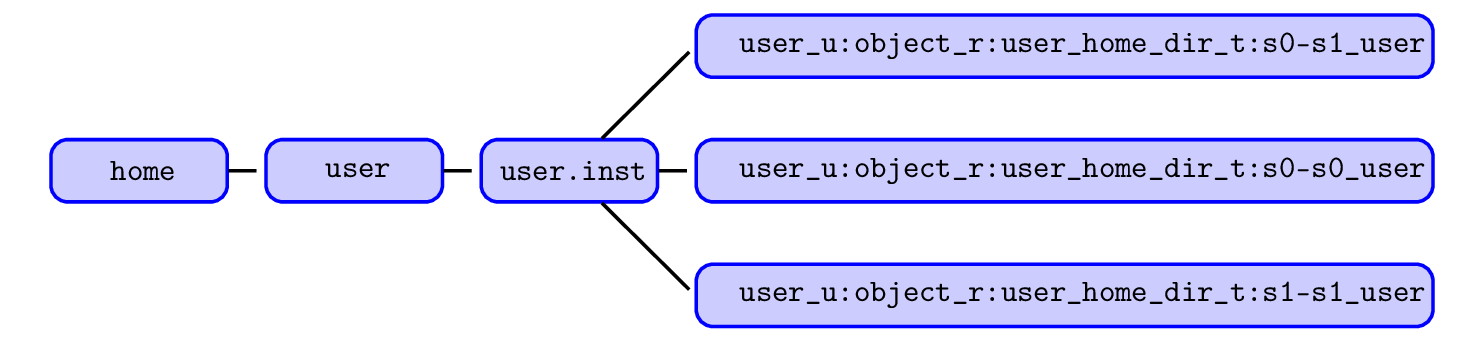
\includegraphics[ scale=0.20]{files/polyinstance.png}
\end{center}

Реализация: модуль pam\_namespace.so\newline
Скрипт инициализации namespace.init\newline
Конфигурационный файл: namespace.conf

\vspace{ 1em }

Реализована:
\begin{itemize}
  \item возможность передачи текущего контекста пользователя в скрипт инициализации
\end{itemize}

  
\end{frame}
\begin{frame}
 \frametitle{OpenSSL}
  

OpenSSL --- Криптографичекский пакет для работы с сертификатами.

\vspace{ 1em }

Дополнения в сертификатах:
\begin{itemize}
  \item Модификация конфигурационного файла openssl.conf
  \item Программно:
\begin{itemize}
  \item alias на существующее дополнение
  \item реализация структуры дополнения
\end{itemize}
\end{itemize}

\vspace{ 1em }

Реализовано:
\begin{itemize}
  \item Дополнение v3\_secon
\end{itemize}

  
\end{frame}
\begin{frame}
 \frametitle{Разработка утилиты создания сертификатов}
  

Требования:
\begin{itemize}
\begin{enumerate}
  \item Возможность создавать закрытый ключ клиента произвольной длины
  \item Создавать запросы на подпись сертификата с дополнением selinuxContext
  \item Подписывать запрос удостоверяющим центром
\end{enumerate}
\end{itemize}

\vspace{1 em }

Реализовано:
\begin{itemize}
  \item утилита на языке Python pgcert
\end{itemize}

  
\end{frame}
\begin{frame}
 \frametitle{sslinfo}
  

sslinfo --- модуль PostgreSQL, предоставляющий возможности просмотра информации о сертификате клиента.

\vspace{1 em}

Расширен:
\begin{itemize}
  \item хранимыми процедурами ssl\_get\_extension\_by\_name(), ssl\_get\_extensions\_count(), ssl\_is\_critical\_extension()
\end{itemize}

  
\end{frame}
\begin{frame}
 \frametitle{Схема стенда}
  

\begin{center}
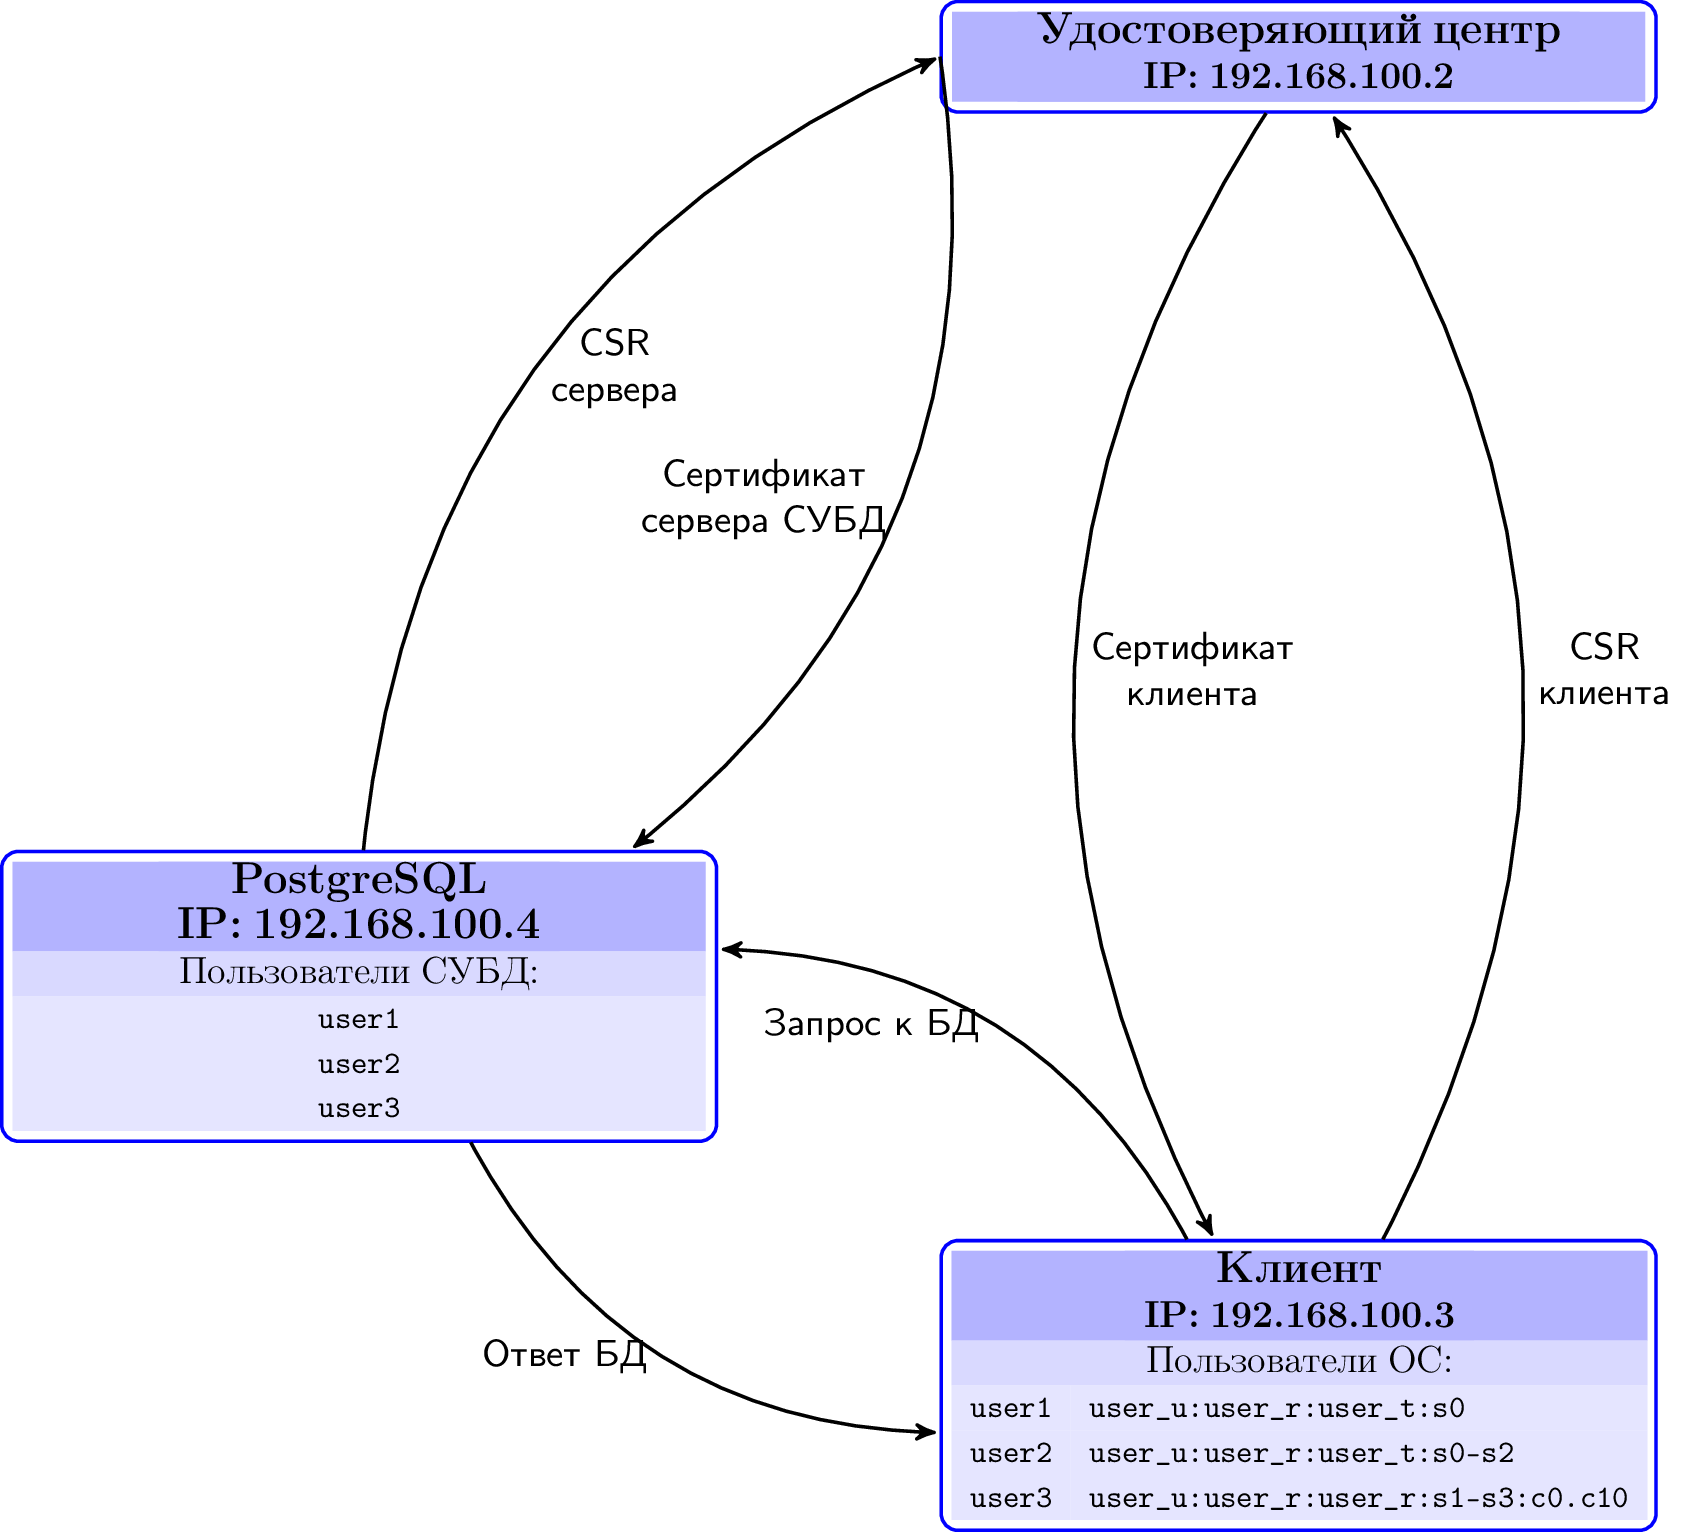
\includegraphics[ scale=0.20]{files/cluster.png}
\end{center}

  
\end{frame}
\begin{frame}
 \frametitle{Тестирование работы механизма}
  

\begin{center}
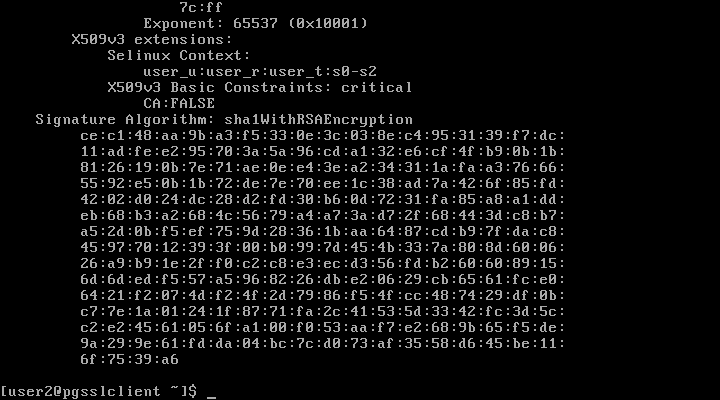
\includegraphics[ scale=0.6]{files/user2_1_4.png}
\end{center}

  
\end{frame}
\begin{frame}
 \frametitle{Тестирование работы механизма}
  

\begin{center}
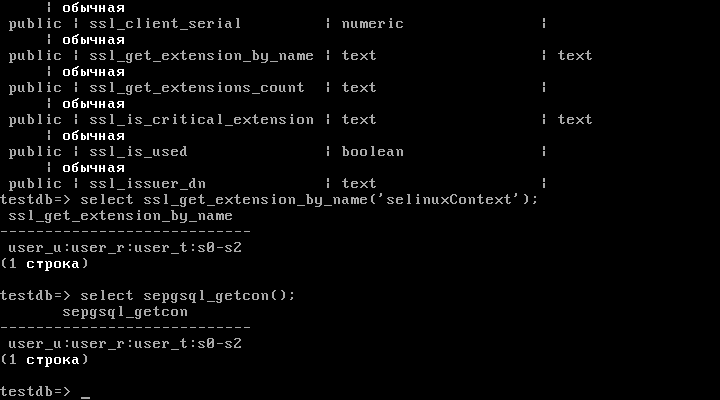
\includegraphics[ scale=0.6]{files/user2_1_7-8.png}
\end{center}

  
\end{frame}
\begin{frame}
 \frametitle{Заключение}
  

\begin{itemize}
  \item Реализован механизм выбора сертификата открытого ключа, содержащего метку безопасности
  \item Расширены возможности pam\_namespace, OpenSSL, M2Crypto, sslinfo
  \item Показано применение разработанного механизма в модуле sepgsql
\end{itemize}

  
\end{frame}
\begin{frame}
 \frametitle{}
  

\begin{center}
Спасибо за внимание!
\end{center}

  
\end{frame}


\end{document}

